\chapter{Multipath Theory and Models}
\label{chap:theory}

\begin{flushright}
 \textit{\textquotedblleft In theory, theory and practice are the same. \\ 
In practice, they are not. \textquotedblright}\\
\textit{--Albert Einstein}
\end{flushright}

\ifpdf
    \graphicspath{{4-Theory/Chapter3Figs/PNG/}{4-Theory/Chapter3Figs/PDF/}{4-Theory/Chapter3Figs/}}
\else
    \graphicspath{{4-Theory/Chapter3Figs/EPS/}{4-Theory/Chapter3Figs/}}
\fi

In this chapter we will start by detailing the various graph algorithms used to compute shortest paths both in the Link State and Distance Vector scenarios. Next, we will describe the concept of Selfish routing which will provide a formal definition of the consequences of congestion insensitive routing. Finally, we will give a brief introduction and present the most remarkable results of Queue Theory which will be used later in this document to model our Multipath routing protocol.

%Then, we will give a description of the flow problems posed by Multipath routing which will provide insight why these algorithms are difficult if not impossible to implement in real networks.

\section{Graph Algorithms}
\label{sect:GraphAlgo}

The algorithms presented in this section do not provide multipath routes but only shortest paths. That said, they can be used, with some minor modifications, to build multipath routes as we will see in Chapter \ref{sect:multiroutes}.

\subsection{Dijkstra's Algorithm}

Dijkstra's Algorithm was proposed by Edsger Dijkstra in 1959 \cite{DIJK}, it is a graph search algorithm which given a graph composed of a set of edges, nodes and edge weights, finds the shortest path from a given source to all other nodes. It is therefore obvious that this algorithm is fundamental in Internet routing.

 The idea behind this algorithm is simple, consider a city's road system with intersections. You wish to find the shortest path between two points in this city. At your start point, you build a list of intersections which are directly connected to it. Then, select the intersection that is closest to your destination and mark the road and the starting intersection used. Next, repeat these steps considering the current intersection as your start point, considering one intersection at each iteration. Once the list of intersections is empty, the algorithm ends, and your shortest path is the the one consisting of all the marked intersections.

We will now give the algorithm description in textual form, the pseudo-code can be found in Section \ref{sect:dijkpseudo}, followed by a running example of the algorithm in Figure \ref{fig:runDijk}, the notation $\frac{x}{y|z}$ is used where x is the node name and y is the distance to the initial node and z the previous node. 

\begin{enumerate}
 \item Set the distance of the initial node to zero and infinity for all the others.
 \item Set all nodes to unvisited except the initial node (current node).
 \item For unvisited neighbors of the current node, compute their distance from the initial node. If this distance is less than their current distance, replace their current distance with the computed one.
 \item Once the distance for all unvisited neighbors have been computed, mark the current node as visited. 
 \item If no unvisited nodes remain, then the algorithm is finished. Otherwise pick the node with the smallest distance from the initial node and set it as the current node and repeat from step 3.
\end{enumerate}

\begin{figure}[!htbp]
\centering

\subfloat[Initial Graph.]{

\begin{tikzpicture}{shorten >=1pt, ->}
  \tikzstyle{every node} = [node distance = 2.5cm,
			    minimum size = 2mm,
			    inner sep = 2,
			    bend angle = 0]
\tikzset{EdgeStyle/.style={->}}
\SetVertexNoLabel
\Vertex{A0}

\NOEA(A0){A1}
\EA(A1){A2}
\SOEA(A0){A3}
\EA(A3){A4}
\AssignVertexLabel{A}{4}{$\frac{A}{0|-}$,$\frac{B}{\infty|-}$,$\frac{C}{\infty|-}$,$\frac{D}{\infty|-}$,$\frac{E}{\infty|-}$}
\tikzstyle{LabelStyle} = [above=6pt]
\Edge[label=$10$](A0)(A1)
\tikzstyle{LabelStyle} = [above=3pt]
\Edge[label=$5$](A0)(A3)
\Edge[label=$1$](A1)(A2)
\Edge[label=$2$](A3)(A4)
\Edge[label=$7$](A4)(A0)
\tikzstyle{LabelStyle} = [above=6pt]
\Edge[label=$9$](A3)(A2)
\tikzset{EdgeStyle/.append style = {bend left = 10}}
\tikzstyle{LabelStyle} = [right=3pt]
\Edge[label=$2$](A1)(A3)
\Edge[label=$4$](A2)(A4)
\tikzstyle{LabelStyle} = [left=3pt]
\Edge[label=$3$](A3)(A1)
\Edge[label=$6$](A4)(A2)

\end{tikzpicture}
}
\hspace{0.3cm}
\subfloat[Search for node closest to A.]{
\begin{tikzpicture}{shorten >=1pt, ->}
  \tikzstyle{every node} = [node distance = 2.5cm,
			    minimum size = 2mm,
			    inner sep = 2,
			    bend angle = 0]
\tikzset{EdgeStyle/.style={->}}
\SetVertexNoLabel
\Vertex{A0}

\NOEA(A0){A1}
\EA(A1){A2}
\SOEA(A0){A3}
\EA(A3){A4}
\AssignVertexLabel{A}{4}{$\frac{A}{0|-}$,$\frac{B}{10|A}$,$\frac{C}{\infty|-}$,$\frac{D}{5|A}$,$\frac{E}{\infty|-}$}
\tikzstyle{LabelStyle} = [above=6pt]
\tikzstyle{EdgeStyle} = [color = red, ->]
\Edge[label=$10$](A0)(A1)
\tikzstyle{LabelStyle} = [above=3pt]
\Edge[label=$5$](A0)(A3)
\tikzstyle{EdgeStyle} = [color = black, ->]
\Edge[label=$1$](A1)(A2)
\Edge[label=$2$](A3)(A4)
\Edge[label=$7$](A4)(A0)
\tikzstyle{LabelStyle} = [above=6pt]
\Edge[label=$9$](A3)(A2)
\tikzset{EdgeStyle/.append style = {bend left = 10}}
\tikzstyle{LabelStyle} = [right=3pt]
\Edge[label=$2$](A1)(A3)
\Edge[label=$4$](A2)(A4)
\tikzstyle{LabelStyle} = [left=3pt]
\Edge[label=$3$](A3)(A1)
\Edge[label=$6$](A4)(A2)

\end{tikzpicture}
}
\hspace{0.3cm}
\subfloat[D found, repeat search for closest node.]{
\begin{tikzpicture}{shorten >=1pt, ->}
  \tikzstyle{every node} = [node distance = 2.5cm,
			    minimum size = 2mm,
			    inner sep = 2,
			    bend angle = 0]
\tikzset{EdgeStyle/.style={->}}
\SetVertexNoLabel
\Vertex{A0}

\NOEA(A0){A1}
\EA(A1){A2}
\SOEA(A0){A3}
\EA(A3){A4}
\AssignVertexLabel{A}{4}{$\frac{A}{0|-}$,$\frac{B}{8|D}$,$\frac{C}{14|D}$,$\frac{D}{5|A}$,$\frac{E}{7|D}$}
\tikzstyle{LabelStyle} = [above=6pt]
\Edge[label=$10$](A0)(A1)
\tikzstyle{LabelStyle} = [above=3pt]
\tikzstyle{EdgeStyle} = [color = green, ->]
\Edge[label=$5$](A0)(A3)
\tikzstyle{EdgeStyle} = [color = black, ->]
\Edge[label=$1$](A1)(A2)
\tikzstyle{EdgeStyle} = [color = red, ->]
\Edge[label=$2$](A3)(A4)
\tikzstyle{EdgeStyle} = [color = black, ->]
\Edge[label=$7$](A4)(A0)
\tikzstyle{LabelStyle} = [above=6pt]
\tikzstyle{EdgeStyle} = [color = red, ->]
\Edge[label=$9$](A3)(A2)
\tikzset{EdgeStyle/.append style = {bend left = 10}}
\tikzstyle{LabelStyle} = [right=3pt]
\tikzstyle{EdgeStyle} = [color = black, ->,bend left = 10]
\Edge[label=$2$](A1)(A3)
\Edge[label=$4$](A2)(A4)
\tikzstyle{LabelStyle} = [left=3pt]
\tikzstyle{EdgeStyle} = [color = red, ->, bend left = 10]
\Edge[label=$3$](A3)(A1)
\tikzstyle{EdgeStyle} = [color = black, ->,bend left = 10]
\Edge[label=$6$](A4)(A2)

\end{tikzpicture}
}
\hspace{0.3cm}
\subfloat[Only consider node C, as others have already been found.]{
\begin{tikzpicture}{shorten >=1pt, ->}
  \tikzstyle{every node} = [node distance = 2.5cm,
			    minimum size = 2mm,
			    inner sep = 2,
			    bend angle = 0]
\tikzset{EdgeStyle/.style={->}}
\SetVertexNoLabel
\Vertex{A0}

\NOEA(A0){A1}
\EA(A1){A2}
\SOEA(A0){A3}
\EA(A3){A4}
\AssignVertexLabel{A}{4}{$\frac{A}{0|-}$,$\frac{B}{8|D}$,$\frac{C}{13|E}$,$\frac{D}{5|A}$,$\frac{E}{7|D}$}
\tikzstyle{LabelStyle} = [above=6pt]
\Edge[label=$10$](A0)(A1)
\tikzstyle{LabelStyle} = [above=3pt]
\tikzstyle{EdgeStyle} = [color = green, ->]
\Edge[label=$5$](A0)(A3)
\Edge[label=$2$](A3)(A4)
\tikzstyle{EdgeStyle} = [color = black, ->]
\Edge[label=$1$](A1)(A2)
\Edge[label=$7$](A4)(A0)
\tikzstyle{LabelStyle} = [above=6pt]
\Edge[label=$9$](A3)(A2)
\tikzset{EdgeStyle/.append style = {bend left = 10}}
\tikzstyle{LabelStyle} = [right=3pt]
\Edge[label=$2$](A1)(A3)
\Edge[label=$4$](A2)(A4)
\tikzstyle{LabelStyle} = [left=3pt]
\tikzstyle{EdgeStyle} = [color = red, ->, bend left = 10]
\Edge[label=$6$](A4)(A2)
\tikzstyle{EdgeStyle} = [color = green, ->, bend left = 10]
\Edge[label=$3$](A3)(A1)

\end{tikzpicture}
}
\hspace{0.3cm}
\subfloat[Consider only C again, for the same reason.]{
\begin{tikzpicture}{shorten >=1pt, ->}
  \tikzstyle{every node} = [node distance = 2.5cm,
			    minimum size = 2mm,
			    inner sep = 2,
			    bend angle = 0]
\tikzset{EdgeStyle/.style={->}}
\SetVertexNoLabel
\Vertex{A0}

\NOEA(A0){A1}
\EA(A1){A2}
\SOEA(A0){A3}
\EA(A3){A4}
\AssignVertexLabel{A}{4}{$\frac{A}{0|-}$,$\frac{B}{8|D}$,$\frac{C}{9|B}$,$\frac{D}{5|A}$,$\frac{E}{7|D}$}
\tikzstyle{LabelStyle} = [above=6pt]
\Edge[label=$10$](A0)(A1)
\tikzstyle{LabelStyle} = [above=3pt]
\tikzstyle{EdgeStyle} = [color = green, ->]
\Edge[label=$5$](A0)(A3)
\Edge[label=$2$](A3)(A4)
\tikzstyle{EdgeStyle} = [color = red, ->]
\Edge[label=$1$](A1)(A2)
\tikzstyle{EdgeStyle} = [color = black, ->]
\Edge[label=$7$](A4)(A0)
\tikzstyle{LabelStyle} = [above=6pt]
\Edge[label=$9$](A3)(A2)
\tikzset{EdgeStyle/.append style = {bend left = 10}}
\tikzstyle{LabelStyle} = [right=3pt]
\Edge[label=$2$](A1)(A3)
\Edge[label=$4$](A2)(A4)
\tikzstyle{LabelStyle} = [left=3pt]
\Edge[label=$6$](A4)(A2)
\tikzstyle{EdgeStyle} = [color = green, ->, bend left = 10]
\Edge[label=$3$](A3)(A1)

\end{tikzpicture}
}
\hspace{0.3cm}
\subfloat[Green edges show the final shortest path graph.]{
\begin{tikzpicture}{shorten >=1pt, ->}
  \tikzstyle{every node} = [node distance = 2.5cm,
			    minimum size = 2mm,
			    inner sep = 2,
			    bend angle = 0]
\tikzset{EdgeStyle/.style={->}}
\SetVertexNoLabel
\Vertex{A0}

\NOEA(A0){A1}
\EA(A1){A2}
\SOEA(A0){A3}
\EA(A3){A4}
\AssignVertexLabel{A}{4}{$\frac{A}{0|-}$,$\frac{B}{8|D}$,$\frac{C}{9|B}$,$\frac{D}{5|A}$,$\frac{E}{7|D}$}
\tikzstyle{LabelStyle} = [above=6pt]
\Edge[label=$10$](A0)(A1)
\tikzstyle{LabelStyle} = [above=3pt]
\tikzstyle{EdgeStyle} = [color = green, ->]
\Edge[label=$5$](A0)(A3)
\Edge[label=$2$](A3)(A4)
\Edge[label=$1$](A1)(A2)
\tikzstyle{EdgeStyle} = [color = black, ->]
\Edge[label=$7$](A4)(A0)
\tikzstyle{LabelStyle} = [above=6pt]
\Edge[label=$9$](A3)(A2)
\tikzset{EdgeStyle/.append style = {bend left = 10}}
\tikzstyle{LabelStyle} = [right=3pt]
\Edge[label=$2$](A1)(A3)
\Edge[label=$4$](A2)(A4)
\tikzstyle{LabelStyle} = [left=3pt]
\Edge[label=$6$](A4)(A2)
\tikzstyle{EdgeStyle} = [color = green, ->, bend left = 10]
\Edge[label=$3$](A3)(A1)

\end{tikzpicture}
}
\caption{Running Example of Dijkstra's Algorithm}
\label{fig:runDijk}
\end{figure}

As is shown by Figure \ref{fig:runDijk}, Dijkstra's Algorithm grows a tree from a given source to all the other nodes for which the distance from the source to all the other nodes is minimal. We initially start with the original graph at node A which has a cost of zero. In the second step, we start at A and search for its closest neighbor (red arrows), we than remove A from the list of unvisited nodes (Q). Next, having found D as the closest neighbor, we can safely mark the edge from A to D as part of the shortest path (green arrow). We then repeat the search for D and find E and remove D from Q. At E we only consider the edge to C as the others link to nodes which are no longer in Q. At the end, we obtain the green graph which is the shortest path from A to all the other nodes. Table \ref{tab:runDijk} shows the intermediate steps in the algorithm, the notation x/y is used where x represents the distance from the initial node and y is the precedent node in the shortest path.

\begin{table}[!htbp]
\begin{center}
\begin{tabular}[]{|c|c|c|c|c|c|c|c|}
$I$ & A   & B          & C          & D          & E         & Q  & Path Nodes \\
0   & 0/- & $\infty/-$ & $\infty/-$ & $\infty/-$ &$\infty/-$ & A-E & $\varnothing$ \\
1   & 0/- & 10/A 	     & $\infty/-$ & 5/A        &$\infty/-$ & B-E & A \\
2   & 	& 8/D 	     & 14/D 	  & 5/A        & 7/D 	   & B,C,E & A,D \\
3   & 	& 8/D 	     & 13/E 	  & 	       & 7/D 	   & B,C & A,D,E \\
4   & 	& 8/D 	     & 9/B 	  & 	       & 	   & C & A,D,E,B \\
5   & 	& 	     	     & 9/B 	  & 	       & 	   & $ \varnothing $ & A,D,E,B,C
\end{tabular}
\end{center}
\caption{Step by Step of Dijkstra's Algorithm}
\label{tab:runDijk}
\end{table}

\subsection{Bellman-Ford Algorithm}

 Bellman-Ford's algorithm \cite{Bellman1958} is the basis for Distance Vector routing protocols. It was proposed simultaneously by Bellman and Ford in 1958. It produces the same result as Dijkstra's algorithm but it is more flexible, namely it allows for negative edge weights\footnote{While this is an interesting fact, it is useless for internet routing. Indeed, negative weights have no physical meaning.}. It is a decentralized algorithm which only requires nodes to inform its neighbors of their distances to other nodes. Then, each node receiving this information picks the shortest advertised weight. 

In a network, routers which use this algorithm maintain a distance table containing an entry for each of the nodes in the network. By looking up in the distance table, a router will know where to send traffic intended for a particular destination. Below we give a textual description of the algorithm, whose pseudo-code can be found in Section \ref{sect:bellpseudo} followed by a running example of the algorithm.

\begin{itemize}
 \item Initialize the graph by setting all distances to $\infty$ and the source's distance to zero.
 \item If the distance from the source to a neighbor using a particular edge is shorter than the current distance, overwrite the current distance with the new one. Repeat this step for all nodes and reconsider all edges in the graph.
 \item Finally check for negative edge cycles by computing the distance from a node to its neighbor, if this distance is smaller than the stored distance then the graph contains negative edge weights.
\end{itemize}

The order in which the edges are visited is not specified by the algorithm, therefore we will opt to visit, from left to right, the top horizontal edges first, then the vertical ones, followed by the bottom horizontal ones, and leave the diagonal ones last. The notation is the same as in the case of Dijkstra. 

\begin{figure}[!htbp]
\centering

\subfloat[Initial Graph]{

\begin{tikzpicture}{shorten >=1pt, ->}
  \tikzstyle{every node} = [node distance = 2.5cm,
			    minimum size = 2mm,
			    inner sep = 2,
			    bend angle = 0]
\tikzset{EdgeStyle/.style={->}}
\SetVertexNoLabel
\Vertex{A0}

\NOEA(A0){A1}
\EA(A1){A2}
\SOEA(A0){A3}
\EA(A3){A4}
\AssignVertexLabel{A}{4}{$\frac{A}{0|-}$,$\frac{B}{\infty|-}$,$\frac{C}{\infty|-}$,$\frac{D}{\infty|-}$,$\frac{E}{\infty|-}$}
\tikzstyle{LabelStyle} = [above=6pt]
\Edge[label=$10$](A0)(A1)
\tikzstyle{LabelStyle} = [above=3pt]
\Edge[label=$5$](A0)(A3)
\Edge[label=$1$](A1)(A2)
\Edge[label=$2$](A3)(A4)
\Edge[label=$7$](A4)(A0)
\tikzstyle{LabelStyle} = [above=6pt]
\Edge[label=$9$](A3)(A2)
\tikzset{EdgeStyle/.append style = {bend left = 10}}
\tikzstyle{LabelStyle} = [right=3pt]
\Edge[label=$2$](A1)(A3)
\Edge[label=$4$](A2)(A4)
\tikzstyle{LabelStyle} = [left=3pt]
\Edge[label=$3$](A3)(A1)
\Edge[label=$6$](A4)(A2)

\end{tikzpicture}
}
\hspace{0.3cm}
\subfloat[At node B, update distances according to edge traversal order]{

\begin{tikzpicture}{shorten >=1pt, ->}
  \tikzstyle{every node} = [node distance = 2.5cm,
			    minimum size = 2mm,
			    inner sep = 2,
			    bend angle = 0]
\tikzset{EdgeStyle/.style={->}}
\SetVertexNoLabel
\Vertex{A0}

\NOEA(A0){A1}
\EA(A1){A2}
\SOEA(A0){A3}
\EA(A3){A4}
\AssignVertexLabel{A}{4}{$\frac{A}{0|-}$,$\frac{B}{8|D}$,$\frac{C}{11|B}$,$\frac{D}{5|A}$,$\frac{E}{7|D}$}
\tikzstyle{LabelStyle} = [above=6pt]
\Edge[label=$10$](A0)(A1)
\tikzstyle{LabelStyle} = [above=3pt]
\tikzstyle{EdgeStyle} = [color = green, ->]
\Edge[label=$5$](A0)(A3)
\Edge[label=$2$](A3)(A4)
\tikzstyle{EdgeStyle} = [color = black, ->]
\Edge[label=$1$](A1)(A2)
\Edge[label=$7$](A4)(A0)
\tikzstyle{LabelStyle} = [above=6pt]
\Edge[label=$9$](A3)(A2)
%\tikzset{EdgeStyle/.append style = {bend left = 10}}

\tikzstyle{EdgeStyle} = [color = green, ->, bend left = 10]
\tikzstyle{LabelStyle} = [left=3pt]
\Edge[label=$3$](A3)(A1)
\tikzstyle{LabelStyle} = [right=3pt]
\tikzstyle{EdgeStyle} = [color = black, ->, bend left = 10]
\Edge[label=$4$](A2)(A4)
\Edge[label=$2$](A1)(A3)
\tikzstyle{LabelStyle} = [left=3pt]
\Edge[label=$6$](A4)(A2)

\end{tikzpicture}
}
\subfloat[Update distance for node C, since it was missed in the last iteration.]{

\begin{tikzpicture}{shorten >=1pt, ->}
  \tikzstyle{every node} = [node distance = 2.5cm,
			    minimum size = 2mm,
			    inner sep = 2,
			    bend angle = 0]
\tikzset{EdgeStyle/.style={->}}
\SetVertexNoLabel
\Vertex{A0}

\NOEA(A0){A1}
\EA(A1){A2}
\SOEA(A0){A3}
\EA(A3){A4}
\AssignVertexLabel{A}{4}{$\frac{A}{0|-}$,$\frac{B}{8|D}$,$\frac{C}{9|B}$,$\frac{D}{5|A}$,$\frac{E}{7|D}$}
\tikzstyle{LabelStyle} = [above=6pt]
\Edge[label=$10$](A0)(A1)
\tikzstyle{LabelStyle} = [above=3pt]
\tikzstyle{LabelStyle} = [above=6pt]
\Edge[label=$10$](A0)(A1)
\tikzstyle{LabelStyle} = [above=3pt]
\tikzstyle{EdgeStyle} = [color = green, ->]
\Edge[label=$5$](A0)(A3)
\Edge[label=$2$](A3)(A4)
\Edge[label=$1$](A1)(A2)
 \tikzstyle{EdgeStyle} = [color = black, ->]
\Edge[label=$7$](A4)(A0)
\tikzstyle{LabelStyle} = [above=6pt]
\Edge[label=$9$](A3)(A2)
%\tikzset{EdgeStyle/.append style = {bend left = 10}}
\tikzstyle{EdgeStyle} = [color = green, ->, bend left = 10]
\tikzstyle{LabelStyle} = [left=3pt]
\Edge[label=$3$](A3)(A1)
\tikzstyle{LabelStyle} = [right=3pt]
\tikzstyle{EdgeStyle} = [color = black, ->, bend left = 10]
\Edge[label=$4$](A2)(A4)
\Edge[label=$2$](A1)(A3)
\tikzstyle{LabelStyle} = [left=3pt]
\Edge[label=$6$](A4)(A2)
\end{tikzpicture}
}

\caption{Running Example of Bellman-Ford's Algorithm}
\label{fig:runBell}
\end{figure}

It may seem in Figure \ref{fig:runBell}, that Bellman-Ford's algorithm is extremely efficient. This is not the case, because for each node it analyses every edge in the network, this is not shown for reasons of brevity and clarity. Bellman-Ford therefore requires  O($|V| |E|$) operations, whereas Dijkstra's algorithm requires O($|E|+ |V|log|V|$), where $|V|$ is the number of vertices's and $|E|$ the number of edges.

%\section{Flow Problems}
%\label{sect:flow}
%nonlinear multicommodity flow problem

%\subsection{Gallager's Algorithm}
%\label{sect:GallagerAlgo}

\section{Selfish Routing}

Selfish routing describes the overall negative effects on the performance of a network when routing decisions are taken selfishly. It is clear that the travel time between two points is highly dependant on the number of users using a given route. Yet, most of us will always opt for the shortest path that gets us to our destination fastest, regardless of the effect this decision has on other users. This is referred to as Selfish Routing \cite{Selfish}.

Routing on the Internet is insensitive to congestion and therefore suffers from the phenomena explained by Selfish routing. Indeed, shortest path routing is analogous to commuters traveling to work each choosing the shortest path and thereby delaying everyone. Figure \ref{fig:pigou} shows a network (referred to as Pigou's Example \cite{Pigou}), in which the total traffic is represented by one, with two paths where the upper one has a delay of one time unit regardless of congestion and the lower path's delay is a function of the congestion. It is reasonable to assume that all traffic will be selfishly routed along the lower path, and therefore that it will be delayed by one time unit. On the other hand, if we consider that the traffic is split equally between the two paths, the overall delay is $\frac{3}{4}$. Indeed, the traffic on the upper path suffers a delay of one time unit but now the traffic on the lower path is only delayed by half a time unit. Therefore, we easily see that no traffic is worse off and moreover half of the traffic is delivered significantly faster. Clearly, the phenomenon illustrated in the first situation could be offset by increasing the link capacities but this is not a tenable nor scalable solution in the longterm.

\begin{figure}[h!]
\begin{center}
\begin{tikzpicture}[>=latex']
 \SetUpEdge[lw         = 2.0pt,
           color      = black],
          labelcolor = black!30],
          labelstyle = {draw,thick,-}]
  %\tikzstyle{edge} = [draw,thick,-]
  \tikzset{node distance = 5.0cm}
  \GraphInit[vstyle=Normal]
  \tikzset{EdgeStyle/.style={->}}
  \tikzset{EdgeStyle/.append style = {bend left = 30}}
  \Vertex{S}
  \EA(S){D}

  \Edge[label=$d(x) {=} 1$](S)(D)
  \tikzset{EdgeStyle/.style={<-}}
  \tikzset{EdgeStyle/.append style = {bend left = 30}}
  \Edge[label=$d(x) {=} x$](D)(S)

\end{tikzpicture}
\end{center}
\caption{Pigou's Example}
\label{fig:pigou}
\end{figure}

%- define a nash flow
%- define optimal flow
%  - price of anarchy worst possible ratio between a selfish routing instance and an optimal instance.
%- define the price of anarchy

Selfish Routing also provides us with a further justification of deploying multipath routing protocols. Before we develop further this justification we must first proceed to the definitions of a few concepts which are more formally detailed in Section \ref{sect:linearanarchy}. First, we must redefine the notion of a flow which will be limited to this section only.

\begin{definition}
  A \emph{flow} $f$ is interpreted as the aggregated routes chosen by the traffic, with $f_p$ measuring the amount of traffic on route $p$.
\end{definition}

\textbf{Note:} The term flow used here differs significantly from our previous definition. This definition only hold for this section and during the rest of this document we will revert to our previous definition.

\begin{itemize}
 \item \emph{Nash Flow} can be seen as a flow routed selfishly, as in the first case given in Figure \ref{fig:pigou}.
 \item \emph{Optimal Flow} is the flow with minimum possible delay, as in the second case of Figure \ref{fig:pigou}.
 \item \emph{Price of Anarchy} is the \emph{worst-possible} ratio between the delay of a Nash flow and that of an optimal flow.
\end{itemize}

With these definitions at hand and if we consider multipath networks with only linear delay functions, Selfish routing tells us that the upper bound\footnote{An upper bound also exists for all polynomial delay functions, which is given in Section \ref{sect:linearanarchy}, but for the sake of clarity we only refer to linear cost functions here.} on the \emph{Price of Anarchy} is $\frac{4}{3}$ (see proof in Section \ref{sect:linearanarchy}). This result further justifies our exploration of multipath networks, because in a multipath network with selfish users it would be expected that additional problems in congestion would arise and therefore deteriorate the performance of the network. This result shows us that this is not the case, and that even in a multipath network with only selfish users there is ``only'' about a 33\% loss in performance, which gives us hope that we may improve the performance of a multipath network significantly while paying a relatively small price in the worst-case scenario (ie. only shortest paths available). Indeed, as we will see in the next chapter, our protocol attempts to leverage all feasible alternative paths and defaults to the shortest path (selfish route) if the alternative paths are not available. As the delay functions increase in degree (ie. polynomial delay functions), the Price of Anarchy increases as well.

%- show that the upper bound for multipath networks is 4/3 --> a 1/3 loss in performance.
%- This shows us that in a multicommodity network, extra obstruction caused by selfish agents do not arise and therefore provides us with an extra justification to proceed in our exploration of a multipath protocol while suggesting that there is yet room for improvement.


\section{Analytical Models}

In this section we present some analytical models based on Queuing Theory which will allow us to model multipath protocols. It should be stated that an exact analysis of multipath communication is too complex \cite{CommNets}, however the independence assumption of Section \ref{sect:kleindep} simplifies the calculations and provides a reasonable approximation. 

\subsection{Queue Theory}
\label{sect:queues}

A queuing system \cite{KLEVol1}, as shown in Figure \ref{fig:queue} is characterized by the following parameters:

\ifigure{queue}{0.5}{A standard queue.}{fig:queue}

\begin{itemize}
 \item \textit{Arrival process (A)} is defined by the distribution of the inter-arrival time of clients into the queue. The only interesting arrival process in this thesis is exponential (Markovian).
 \item \textit{Service time distribution (B)} represents the time required to serve a client present at the top of the queue. We will only deal with Markovian distributions.
 \item \textit{Number of servers (m)} present in a single queue. We will deal with models containing one or more servers.
 \item \textit{Capacity (K)} of the queue is the maximum number of clients which can be present in the system at any given moment.
 \item \textit{Population size (N)} represents the potential number of clients whether finite or infinite. We will consider situations with infinite populations.
 \item \textit{Queuing policy (D)} defines in which order the next client is selected from the queue, eg. first in, first out (FIFO).
\end{itemize}

\textit{Kendall's Notation} is often used to identify the type of queue used which is denoted by A/B/m/K/N/D. The parameters K, N, and D are often omitted indicating that they are either infinite or that a FIFO policy is used. 

The arrival and service time processes can be either of the following:

\begin{itemize}
 \item \textit{Markovian} - A Poisson distribution \cite{Poisson} where the inter-arrival times are independent and exponentially distributed.
 \item \textit{Deterministic} - constant inter-arrival/service time.
 \item \textit{General Distribution} where the underlying probability density function is arbitrary.
\end{itemize}

It is worth presenting some general results and notations which apply to all queuing systems:

\begin{itemize}
 \item $\lambda$ is the average inter arrival rate of clients into the systems.
 \item $\frac{1}{\mu}$, the average service time per server.
 \item $\rho$ is the utilization factor of the queue ($\frac{\lambda}{\mu}$ and $\frac{\lambda}{m\mu}$ in the multi-server case). For the queue to be stable, we should have $0 \leq \rho < 1$.
\item $T$ is the total average time in the system (queue + service).
\begin{equation}
 T = W + \frac{1}{\mu} = \frac{1}{\mu - \lambda}
 \label{eq:GG1T}
\end{equation}
 \item $W$ is the average waiting time in the queue.
 \begin{equation}
 W = \frac{\rho}{\mu - \lambda}
 \label{eq:GG1W}
\end{equation}
 \item $\bar{N}$ is the average number of clients in the system given by Little's Result \cite{little}.
\begin{equation}
  \bar{N} = \lambda T
 \label{eq:Little}
\end{equation}
 \item $\bar{N}_q$ is the average size of the queue.
\begin{equation}
 \bar{N}_Q = \bar{N} - m\rho
 \label{eq:GG1NQ}
\end{equation}

 
 \item $P_N$ is the probability that there are N clients in the system.
\end{itemize}

In the next sections we will present remarkable results for both the M/M/1 and M/M/m queues. We will also describe Kleinrock's Independence Assumption. 

\subsubsection{M/M/1 Queue}

The M/M/1 queue is composed of exponentially distributed inter-arrival process and service times along with a single server model. The M/M/1 queue is the simplest form a queue can take, while still remaining interesting. While being simple its behavior is similar to other more complex cases. 

Since the inter arrival distribution is Poisson, the arrival rate is given by $\lambda$ and the service time is $\frac{1}{\mu}$, which gives us directly the following relations:

\begin{equation}
\bar{N} = \frac{\rho}{1-\rho}
\label{eq:MM1N}
\end{equation}
 
Using Little's Result (Equation \ref{eq:Little}) and Equation \ref{eq:GG1NQ}, we obtain the following relations for $W$ and $T$.

\begin{equation}
W = \frac{\rho}{\mu(1-\rho)} 
\label{eq:MM1W}
\end{equation}

and,

\begin{equation}
T = \frac{1}{\mu(1-\rho)}
\label{eq:MM1T}
\end{equation}

\begin{figure}[htbp!]
\begin{center}

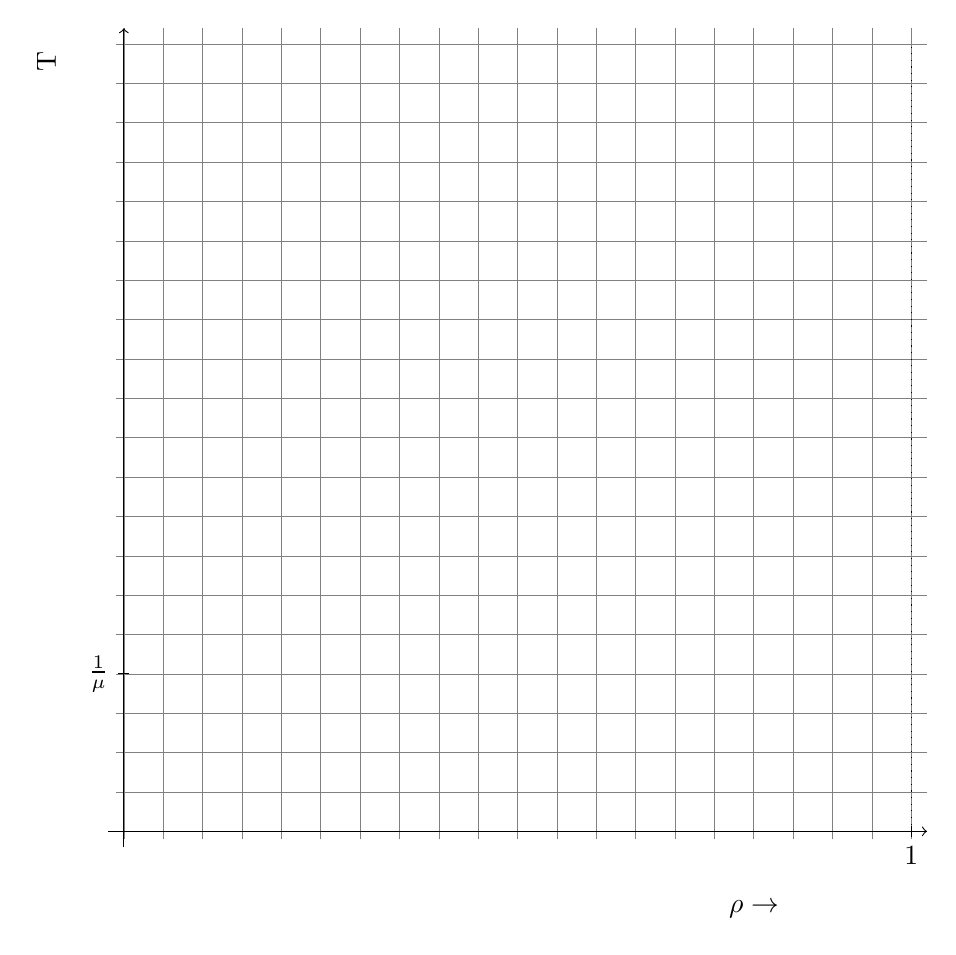
\begin{tikzpicture}[scale=1.0, domain=0:9.8]
    \draw[very thin,color=gray,step=.5cm] (-0.1,-0.1) grid (10.2,10.2);
    \draw[->] (-0.2,0) -- (10.2,0) node[below = 28pt, left=50pt] {$\rho \rightarrow$};
    \draw[->] (0,-0.2) -- (0,10.2) node[left = 28pt, below=5pt] {$\rotatebox{90}{T}$};
    \draw[dotted](10,0) -- (10,10);
    \foreach \x/\xtext in {10/1}
      \draw[shift={(\x,0)}] (0pt,2pt) -- (0pt,-2pt) node[below] {$\xtext$};
    \foreach \y/\ytext in {2/\frac{1}{\mu}}
    \draw[shift={(0,\y)}] (2pt,0pt) -- (-2pt,0pt) node[left] {$\ytext$};

%MODIFIED BY HAND

    \draw[color=black] plot[id=delay] function{(1/(1-(x/10)))};


\end{tikzpicture}
\end{center}
\caption{Average delay as a function of $\rho$.}
\label{fig:MM1INF}
\end{figure}

%\ifigure{MM1INF}{0.8}{Average delay as a function of $\rho$.}{fig:MM1INF}

All the relations given for $\bar{N}$, $T$, and $W$ demonstrate common behavior with respect to the utilization factor $\rho$, more precisely they behave inversely to $1 - \rho$. Therefore, as $\rho$ tends towards one the average delays and queue sizes tend towards infinity as shown in Figure \ref{fig:MM1INF}.


\subsubsection{M/M/m Queue}
\label{sect:mmmQ}

We will now consider a generalization of the M/M/1 queue to m servers. In this model, a single queue forms the entry to the system and a collection of servers will handle the first client at the head of the queue. As previously, $\lambda$ is the arrival rate and $\frac{1}{\mu}$ is the average service time. Also, we have here that $\rho = \frac{\lambda}{m\mu}$.

Before presenting the steady state relations relative to an M/M/m queue, we must first distinguish the situations where the queue is busy and when it is not, which help establish the steady state relations. This is given by the probability of finding that all servers are busy when a new client arrives:

\begin{equation}
P_{Q} = \frac{p_{0}(m\rho)^{m}}{m!(1-\rho)}
\label{eq:MMMPQ}
\end{equation}

where,

\begin{equation}
p_{0} = \left[ \displaystyle\sum\limits_{n=0}^{m-1} \frac{(m\rho)^{n}}{n!} + \frac{(m\rho)^{m}}{m!(1-\rho)}\right]^{-1}
\label{MMMP0}
\end{equation}

$P_{Q}$ is known as the \emph{Erlang C formula} \cite{Erlang} and is widely used in telephony. Now we give the following relations for the number of clients in the system and in the queue, respectively. The complete derivation of these relations can be found in cite{KLEVol1} and other Queuing Systems literature, the author only wishes to remind them here.

\begin{equation}
 \bar{N} = m\rho + \frac{\rho P_{Q}}{1-\rho}
\label{eq:MMMN} 
\end{equation}

and,

\begin{equation}
\bar{N}_Q = \frac{\rho P_{Q}}{1 - \rho}
\label{eq:MMMNQ} 
\end{equation}


Using Little's Result (Equation \ref{eq:Little}) and Equation \ref{eq:GG1NQ}, we obtain the following relations for the average time (network delay) and the average waiting time (forwarding and processing time) spent in the system, respectively.

\begin{equation}
 T = \frac{1}{\mu}\left(1 + \frac{P_{Q}}{m(1-\rho)}\right)
\label{eq:MMMT} 
\end{equation}

and,

\begin{equation}
 W = \frac{P_{Q}}{m\mu\left(1-\rho\right)}
\label{eq:MMMW} 
\end{equation}
%\subsubsection{Jackson's Theory - Networks of Queues}

\subsubsection{Kleinrock's Independence Assumption}
\label{sect:kleindep}
% ------------------------------------------------------------------------
In the two models, presented above, we have assumed that both the arrival and service times respect the Markovian property, ie. the future state of the system depends only on the present state. Moreover Burke's Theorem \cite{Burke} states:

\newtheorem{theorem}{Theorem}
\begin{theorem}
\label{th:Burke}
\textbf{Burke's Theorem.} The steady-state output of a queue with N channels in parallel, with Poisson arrivals and message lengths chosen independently from an exponential distribution is itself Poisson-distributed. 
\end{theorem}

Consider now the situation, which exists within data networks, where many queues interact in the sense that the output from one queue is the input of another (or possibly several others). Given Burke's Theorem and the models we have presented, one might think that delays in data networks are simple to obtain via such models. Unfortunately this is not the case, the message (or packet) inter-arrival time and the message lengths beyond the first queue in the network become strongly dependent. Due to the fact that the service times at each queue are a function of the message length and therefore the arrival time at each subsequent queue is no longer Markovian \cite{CommNets}.

%\ifigure{tandem}{0.7}{A tandem network.}{fig:tandem}

\tikzstyle{vertex}=[circle,fill=black,minimum size=10pt,inner sep=0pt]
\tikzstyle{texver} = [circle, fill=black!25, minimum size = 20pt]
\tikzstyle{edge} = [draw,thick,->]

\begin{figure}[htbp!]
\begin{center}
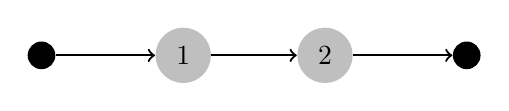
\begin{tikzpicture}[scale=1.8, auto,swap]
 \foreach \pos/\name in {{(0,0)/0}, {(3,0)/3}}
        \node[vertex]   (\name) at \pos {};
        
  \foreach \pos/\name in {{(1,0)/1}, {(2,0)/2}}
        \node[texver] (\name) at \pos {$\name$};

\foreach \source/ \dest in {0/1,1/2,2/3}
        \path[edge] (\source) -- (\dest);
	

\end{tikzpicture}
\caption{A tandem network.}
\label{fig:tandem}
\end{center}
\end{figure}


Figure \ref{fig:tandem} illustrates two queues in tandem where packet lengths are exponentially distributed and independent of each other as well as the inter-arrival times at the first queue. We can therefore state that the first queue follows the M/M/1 model, but we cannot say the same about the second queue because the inter-arrival times at the second queue are strongly correlated with the packets lengths. Indeed the inter-arrival time at the second queue is \textbf{equal} to the transmission time at the first queue. As an analogy to this situation, consider a truck traveling on a narrow busy road along with several fast cars. Typically the truck will see an empty road ahead of it while it is being closely followed by a line of cars. The dependence between inter-arrival and message lengths (and therefore service time) is a source of great mathematical complexity for the analysis of queuing networks, in which even the simple case of the tandem network has no known exact solution \cite{DataNetworks}. A full mathematical demonstration of this dependence is given in Section \ref{sect:KLEDEP}.

As previously shown the dependence appears for queues which are internal to the network. Therefore, one might ask: Why is there a difference between the initial (network entry) queue and internal queues? The answer is straightforward, the initial queue receives its messages from an external source consisting of many subscribers (in our case people or computers) which are all generating messages. The overall message generation by the subscribers exhibits an independence \cite{CommNets} since one message is different from one person to the next. In a general network a similar situation exists. Indeed, more than one queue can deliver messages to any given queue, similarly any given queue is receiving messages from many other queues. If we accept this observation then we can define the following assumption:

%\newtheorem{}{Theorem}
\begin{theorem}
\label{th:indep}
\textbf{Independence Assumption.} Each time a message is received at a queue within the net, a new length $v$ is chosen for this message from the following distribution:

\begin{center}
 $P(v) = \mu e^{-\mu v}$
\end{center} 
\end{theorem}

Obviously, such an assumption does not correspond to the reality with a general network. Nevertheless, it results in a far simpler mathematical modeling of networks, while still maintaining an acceptable degree of accuracy \cite{CommNets}. 


\section{Summary}

This section has presented the modeling tools that we have used to describe our protocols. As we have shown, it is clearly beyond the scope of this document to attempt to describe multipath networks accurately due to the sheer mathematical complexity involved. 

We have also discussed and given justification for deploying multipath protocols. While the use of multipath may seem evident, using longer paths rather than only the shortest path is less clear. We have seen that routing selfishly (ie. always onto the shortest path), causes the performance to drop significantly.
%%% Local Variables: 
%%% mode: latex
%%% TeX-master: "../thesis"
%%% End: 
